\documentclass{beamer}
\usepackage{beamerthemeshadow}
\usepackage[ruled]{algorithm}
\usepackage{listings}
\usepackage[font=scriptsize]{subcaption}
\usepackage[font=scriptsize]{caption}
\usepackage[noend]{algpseudocode}

%\graphicspath{ {../data/figures/} }


\begin{document}
\title{A Lock-free Priority Queue Design Based on Multi-dimensional Linked Lists}
\author[D. Zhang \and D. Dechev]{Deli Zhang \and Damian Dechev}
\institute{University of Central Florida}
\date{\today}

\begin{frame}
    \titlepage
\end{frame}

%\begin{frame}
    %\frametitle{Table of Contents}
    %\tableofcontents
%\end{frame}

\section{Background}
\subsection{Motivation}
\begin{frame} \frametitle{Priority Queues}
    \begin{itemize}
        \item Abstract Data Structure
            \begin{itemize}
                \item \texttt{Insert} adds a key-value pair into the queue sorted by keys
                \item \texttt{DeleteMin} returns and removes the first key-value pair
            \end{itemize}
        \item Typical Sequential Implementations
            \begin{itemize}
                \item Balanced Search Trees
                \item Array-based Binary Heap
            \end{itemize}
    \end{itemize}
\end{frame}

\begin{frame} \frametitle{Concurrent Priority Queues}
    \begin{itemize}
        \item Skip-list
            \begin{itemize}
                \item Use randomization to avoid global balancing
                \item Keep redundant short-cut lists for fast search
            \end{itemize}
        \item Skip-list based approaches
            \begin{itemize}
                \item Sundell et al. 2005: first lock-free linearizable implementation 
                \item Shavit et al. 2009: lock-free and quiescently consistent
                \item Linden et al 2013: batch physical deletion to reduce contention 
                %\item Alistarh and Shavit 2014: Relaxed \texttt{DeleteMin}
            \end{itemize}
    \end{itemize}
\begin{figure}[H]
                \centering
                \includegraphics<1>[width=1\textwidth]{./Skip_list_svg.png}
            \end{figure}
\end{frame}

\section{Algorithm}
\subsection{Overview}
\begin{frame} \frametitle{Ordered Linked List}
\begin{columns}
        \begin{column}{7cm}
            \begin{figure}[H]
                \centering
                \includegraphics<1>[width=1\textwidth]{./mdlist-1d.pdf}
            \end{figure}
        \end{column}
        \begin{column}{5cm}
            \begin{itemize}
                \item $\mathcal{O}(n)$ search/insertion
                \item $\mathcal{O}(1)$ deletion
            \end{itemize}
        \end{column}
    \end{columns}
\end{frame}

\begin{frame} \frametitle{Ordered 2-D List}
\begin{columns}
        \begin{column}{7cm}
            \begin{figure}[H]
                \centering
                \includegraphics<1>[width=1\textwidth]{./mdlist-2d.pdf}
            \end{figure}
        \end{column}
        \begin{column}{5cm}
            \begin{itemize}
                \item Vector $(d_0, d_1)$ serves as insertion coordinates
                \item $\mathcal{O}(\sqrt n)$ search/insertion
                \item $\mathcal{O}(1)$ deletion
            \end{itemize}
        \end{column}
    \end{columns}
\end{frame}

\begin{frame} \frametitle{Multi-dimensional List}
    \begin{definition}
    A $D$-dimensional list is a rooted tree in which each node is implicitly assigned a dimension of $d \in [0,D)$. The root node's dimension is $0$. A node of dimension $d$ has no more than $D-d$ children, where the $m$th child is assigned a dimension of $d'=d+m-1$.
    \end{definition}
    \begin{definition}
    Given a non-root node of dimension $d$ with coordinate $\mathbf{k}=(k_0,...,k_{D-1})$ and its parent with coordinate $\mathbf{k'}=(k'_0,...,k'_{D-1})$ in an ordered $D$-dimensional list: $k_i = k'_i, \;\forall \;i \in [0, d) \land k_d > k'_d$.
    \end{definition}
\end{frame}

\begin{frame} \frametitle{Ordered 3-D List}
\begin{columns}
        \begin{column}{7cm}
            \begin{figure}[H]
                \centering
                \includegraphics<1>[width=1\textwidth]{./mdlist-3d.pdf}
            \end{figure}
        \end{column}
        \begin{column}{5cm}
             \begin{itemize}
                \item Worst-case $\mathcal{O}(D \sqrt[D]{n})$ search/insertion
                \item Choose $D = \log{n}$ then $\log{n} \sqrt[\log{n}]{n} = \mathcal{O}(\log{n})$
                \item No need for global re-balancing/randomization
            \end{itemize}           
        \end{column}
    \end{columns}
\end{frame}

\subsection{Insertions}
\begin{frame} \frametitle{Locate Unique Inserting Position}
\begin{columns}
        \begin{column}{7cm}
            \begin{figure}[H]
                \centering
                \includegraphics<1>[width=1\textwidth]{./mdlist-3d-ins-1.pdf}
            \end{figure}
        \end{column}
        \begin{column}{5cm}
            \begin{itemize}
                \item Compare coordinate vector from $d=0$
                \item Increase $d$ if equal
                \item Go to $d$th child if greater 
                \item Stop if smaller
            \end{itemize}
        \end{column}
    \end{columns}
\end{frame}

\begin{frame} \frametitle{Insert}
\begin{columns}
        \begin{column}{7cm}
            \begin{figure}[H]
                \centering
                \includegraphics<1>[width=1\textwidth]{./mdlist-3d-ins-2.pdf}
            \end{figure}
        \end{column}
        \begin{column}{5cm}
            \begin{itemize}
                \item Point to parent's old child
                \item Update parent's child pointer
                \item Adopt old child's children if old child's dimension is changed
            \end{itemize}
        \end{column}
    \end{columns}
\end{frame}

\begin{frame} \frametitle{Adopting Children}
\begin{columns}
        \begin{column}{7cm}
            \begin{figure}[H]
                \centering
                \includegraphics<1>[width=1\textwidth]{./mdlist-3d-ins-3.pdf}
            \end{figure}
        \end{column}
        \begin{column}{5cm}
            \begin{itemize}
                \item New node $d=0$
                \item Old child $d=2$
                \item Old child's children on dimension 0, 1 are transfer to new node
            \end{itemize}
        \end{column}
    \end{columns}
\end{frame}

\subsection{DeleteMin}
\begin{frame} \frametitle{Normal Deletion}
\begin{columns}
        \begin{column}{7cm}
            \begin{figure}[H]
                \centering
                \includegraphics<1>[width=1\textwidth]{./mdlist-3d-del-1.pdf}
            \end{figure}
        \end{column}
        \begin{column}{6cm}
            \begin{itemize}
                \item Prompt the next minimal node 
                \item Preserve two children
            \end{itemize}
        \end{column}
    \end{columns}
\end{frame}

\begin{frame} \frametitle{Normal Deletion - Promotion}
\begin{columns}
        \begin{column}{7cm}
            \begin{figure}[H]
                \centering
                \includegraphics<1>[width=1\textwidth]{./mdlist-3d-del-2.pdf}
            \end{figure}
        \end{column}
        \begin{column}{6cm}
            \begin{itemize}
                \item Transfer them to the new head
                \item Heavy contention on the head nodes
            \end{itemize}
        \end{column}
    \end{columns}
\end{frame}

\begin{frame} \frametitle{Stack-based Deletion}
\begin{columns}
        \begin{column}{7cm}
            \begin{figure}[H]
                \centering
                \includegraphics<1>[width=1\textwidth]{./mdlist-3d-stack-1.pdf}
            \end{figure}
        \end{column}
        \begin{column}{5cm}
            \begin{itemize}
                \item Mark for logical deletion
                \item DPS to find next node
                \item Use stack as cache to DPS path
            \end{itemize}
        \end{column}
    \end{columns}
\end{frame}

\begin{frame} \frametitle{Stack-based Deletion}
\begin{columns}
        \begin{column}{7cm}
            \begin{figure}[H]
                \centering
                \includegraphics<1>[width=1\textwidth]{./mdlist-3d-stack-2.pdf}
            \end{figure}
        \end{column}
        \begin{column}{5cm}
            \begin{itemize}
                \item Mark for logical deletion
                \item DPS to find next node
                \item Use stack as cache to DPS path
            \end{itemize}
        \end{column}
    \end{columns}
\end{frame}

\subsection{Concurrent Access}
\begin{frame} \frametitle{Lock-free Priority Queue}
    \begin{itemize}
        \item Concurrent Insertion
            \begin{itemize}
                \item Use CAS to swing predecessor's pointer
                \item Use descriptor that resides in the node to finish the children adoption process
            \end{itemize}
        \item Concurrent DeleteMin
            \begin{itemize}
                \item Deletion threads use \emph{deletion stack} to find the next node
                \item Deletion threads move stack forward, and purge deleted nodes
                \item Insertion threads rewind stack if new node cannot be reached 
            \end{itemize}
    \end{itemize}
\end{frame}

\subsection{Correctness}
\begin{frame} \frametitle{Abstract State Mapping}
    \begin{figure}[h]
        \centering
        \includegraphics<1>[width=0.8\textwidth]{./mdlist-abstract_state.pdf}
    \end{figure}
    \begin{figure}[h]
        \centering
        \includegraphics<1>[width=0.8\textwidth]{./mdlist-purge.pdf}
    \end{figure}
\end{frame}


\section{Experimental Evaluation}
\subsection{Performance Testing}
\begin{frame} \frametitle{Throughput}
\begin{figure}[t]
    \begin{subfigure}{0.3\textwidth}
        \centering
        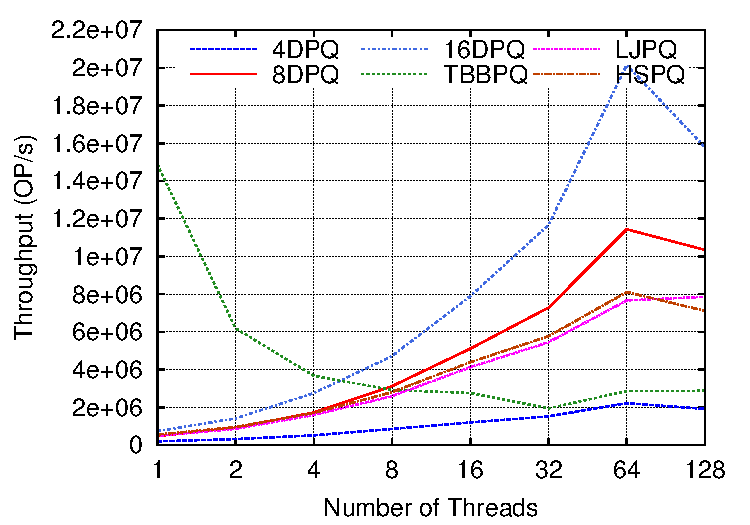
\includegraphics[width=1\columnwidth]{../data/amd100insertion.pdf}
        \caption{100\% \textsc{Insert} on the NUMA System}
        \label{fig:100ins}
    \end{subfigure}
    \hfill
    \begin{subfigure}{0.3\textwidth}
        \centering
        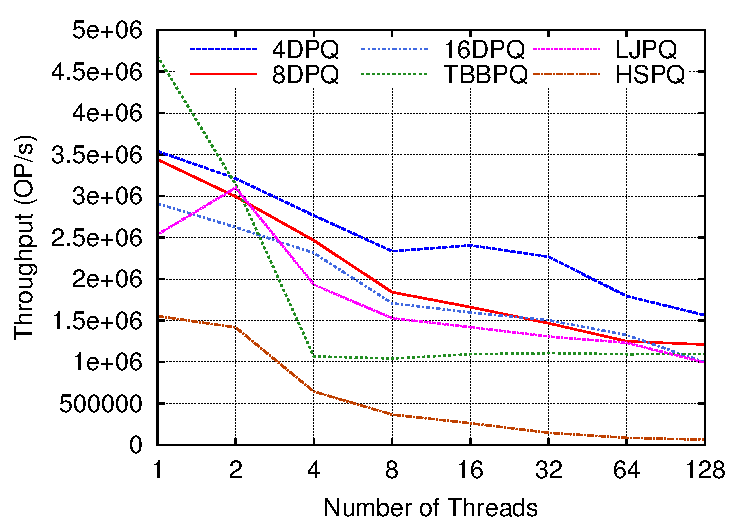
\includegraphics[width=1\columnwidth]{../data/amd0insertion.pdf}
        \caption{100\% \textsc{DeleteMin} on the NUMA System}
        \label{fig:0ins}
    \end{subfigure}
    \hfill
    \begin{subfigure}{0.3\textwidth}
        \centering
        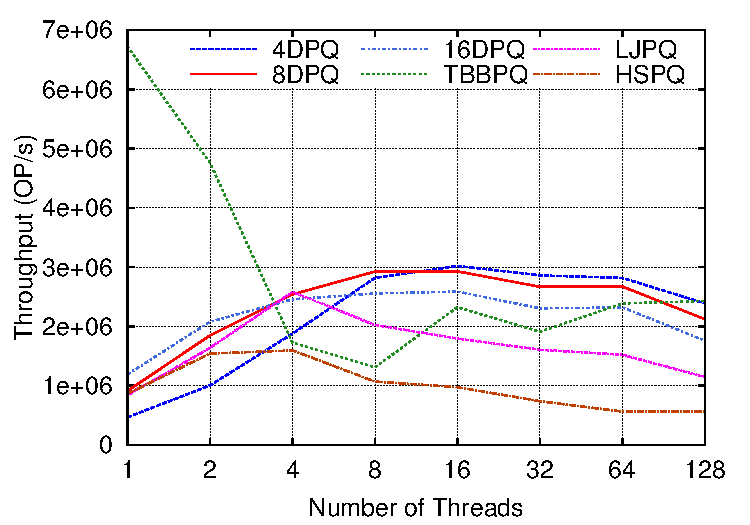
\includegraphics[width=1\columnwidth]{../data/amd50insertion.pdf}
        \caption{50\% \textsc{Insert} on the NUMA System}
        \label{fig:50ins}
    \end{subfigure}
    \begin{subfigure}{0.3\textwidth}
        \centering
        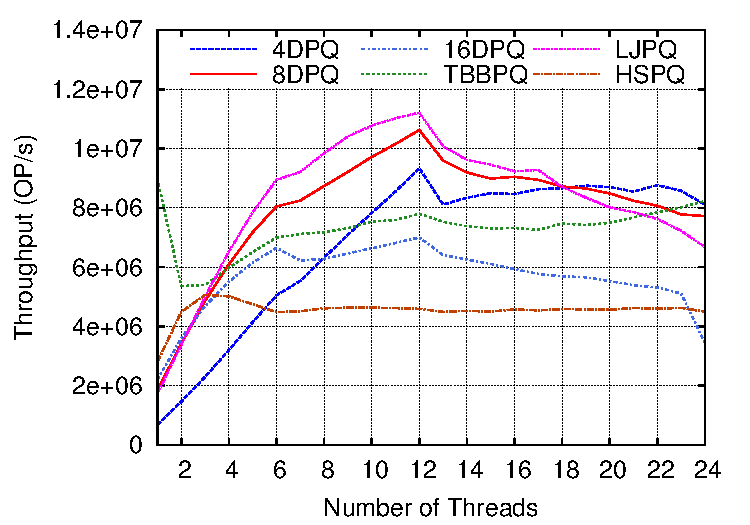
\includegraphics[width=1\columnwidth]{../data/intel50insertion.pdf}
        \caption{50\% \textsc{Insert} on the SMP System}
        \label{fig:50insintel}
    \end{subfigure}
    \hfill
    \begin{subfigure}{0.3\textwidth}
        \centering
        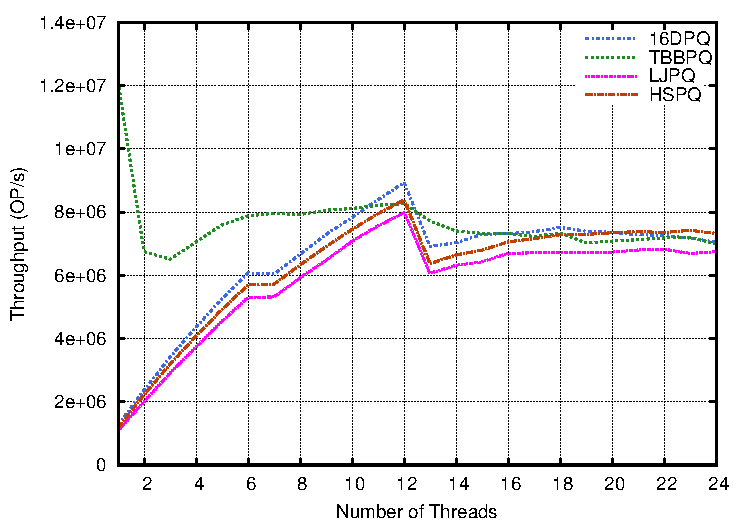
\includegraphics[width=1\columnwidth]{../data/intel80insertion.pdf}
        \caption{80\% \textsc{Insert} on the SMP System}
        \label{fig:80ins}
    \end{subfigure}
    \hfill
    \begin{subfigure}{0.3\textwidth}
        \centering
        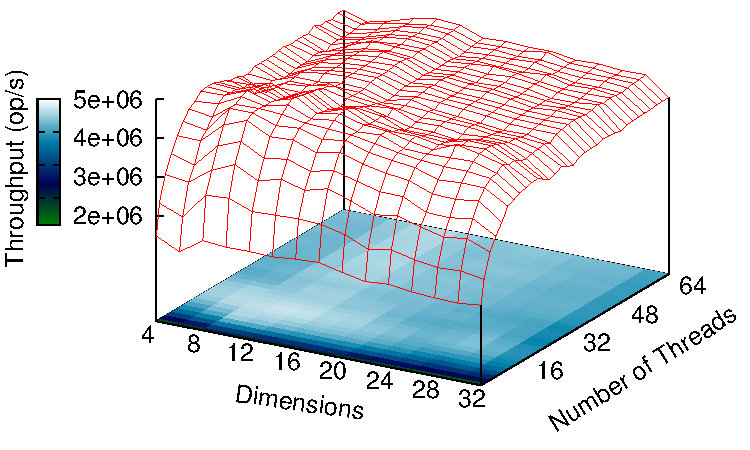
\includegraphics[width=1\columnwidth]{../data/amdsweep75insert.pdf}
        \caption{Dimensionality and Performance}
        \label{fig:sweep}
    \end{subfigure}
    \caption{Throughput of the Priority Queues}
    \label{fig:throughput}
\end{figure}
\end{frame}

%\section{Conclusion}
%\begin{frame} \frametitle{Comments}
    %\begin{itemize}
        %\small
        %\item Todo: fix a bug that nodes are sometimes missing after insertion
        %\item Todo: integrate Sundell's approach for further testing
        %\item Insight: high dimension for more tree like behavior - faster insertions
        %\item Insight: low dimension for more list like behavior - faster deletions
        %\item Application: Priority Queue, Dictionary, Sparse vector
    %\end{itemize}
%\end{frame}

%\begin{frame}
    %\begin{center}
        %\large
%Questions? \\
%\bigskip
%Thank you!
    %\end{center}
%\end{frame}

\end{document}
